\begin{figure*}
    \centering
    % 第一张子图及图注
    \begin{subfigure}[t]{0.47\textwidth}
        \centering
        \resizebox{\textwidth}{!}{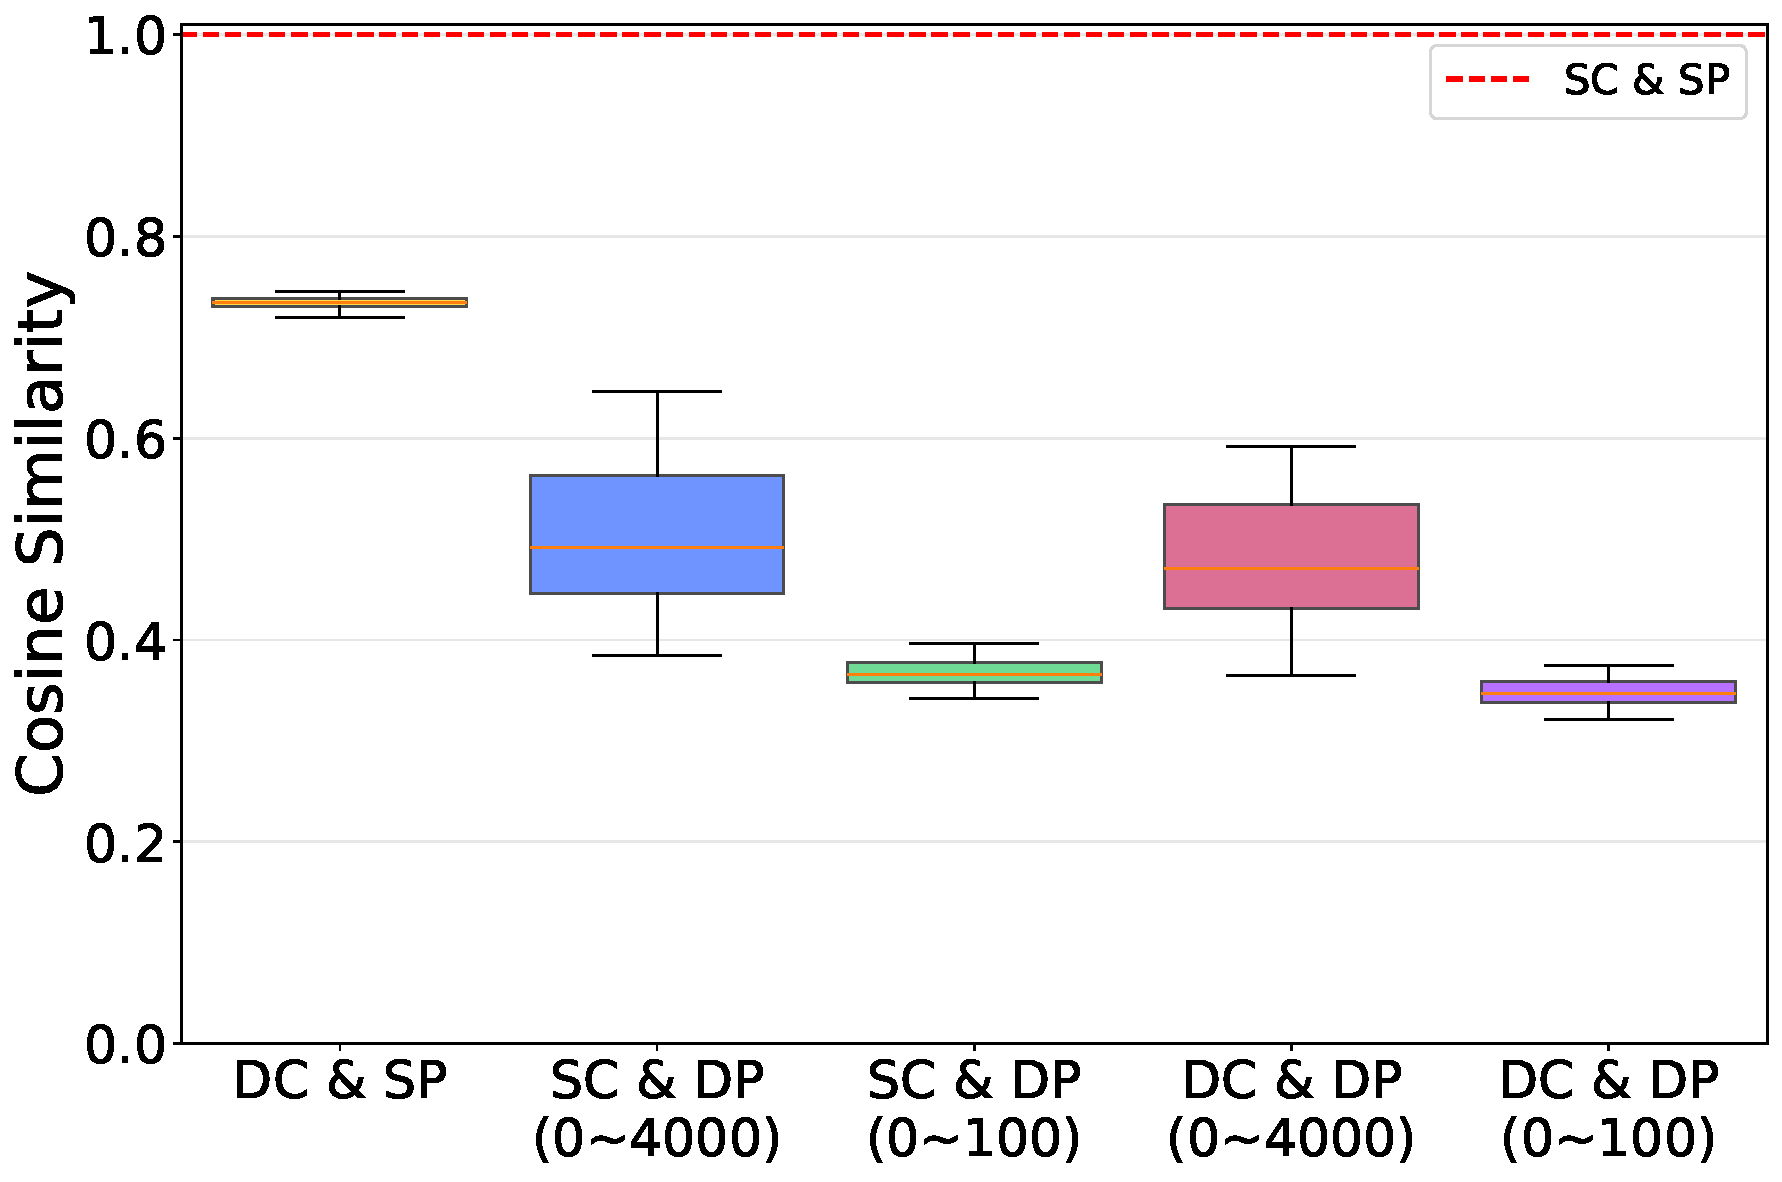
\includegraphics{images/similarity_boxplot.pdf}}
        % \caption{Boxplot of query similarity distributions.}  % 第一张图的图注
        \caption{}  % 第一张图的图注
        \label{fig:query_similarity_boxplot}
    \end{subfigure}
    \hspace{0.5cm}  % 两图间距
    % 第二张子图及图注
    \begin{subfigure}[t]{0.47\textwidth}
        \centering
        \resizebox{\textwidth}{!}{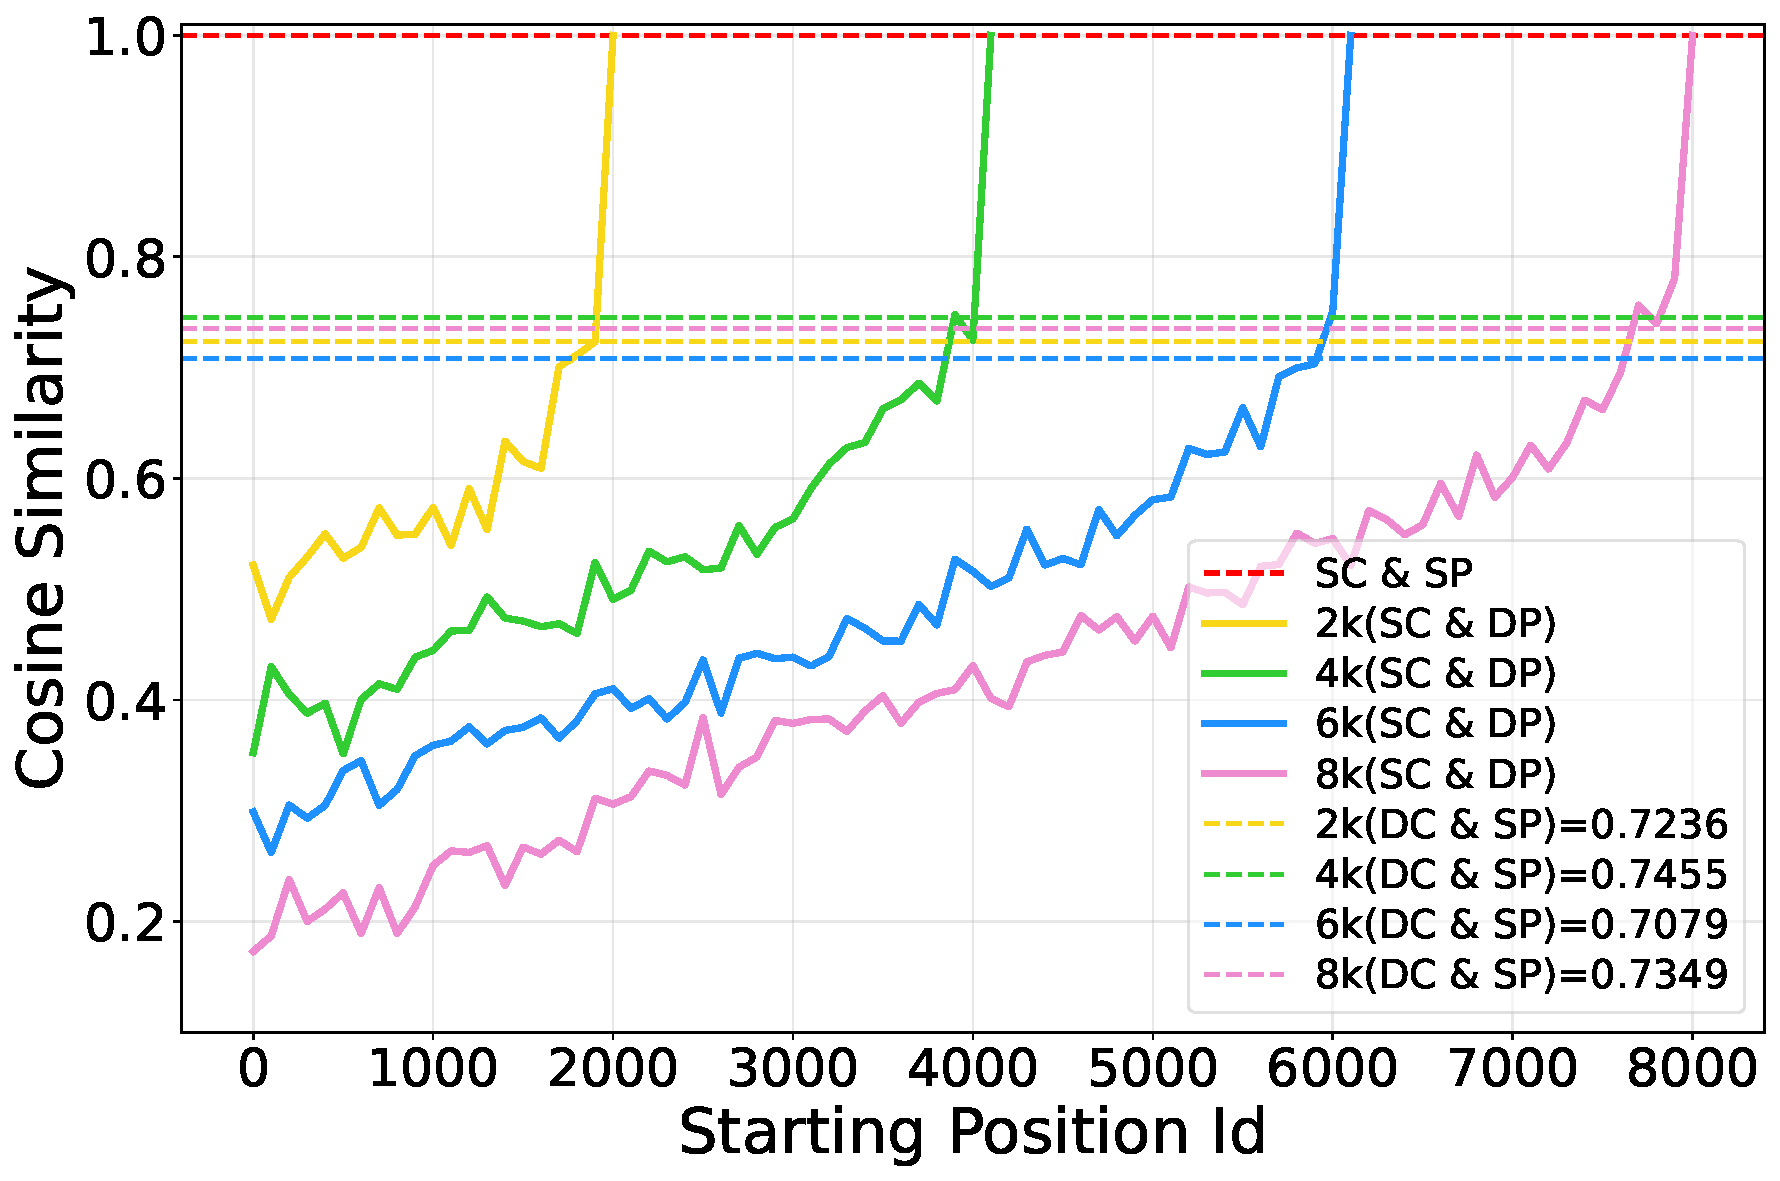
\includegraphics{images/average_similarity_curve.pdf}}
        % \caption{Curve of query similarity over offset positions.}  % 第二张图的图注
        \caption{}
        \label{fig:query_similarity_curve}
    \end{subfigure}
    \vspace{-7pt}
    % 可选总标题（概括两图内容）
    \caption{Analysis of Positional Dominance and Offset Sensitivity in Query Similarity. We set the pseudo queries of fixed length 32. (a) Boxplot of query similarity distributions for a 4k context under different content and position conditions, each aggregated from 100 independent trials. DC: pseudo-queries content is constructed by randomly sampling 32 tokens from the model's vocabulary; DP: pseudo-queries positions are assigned by randomly sampling a consecutive span of 32 index positions from the context length range [0, m] (e.g., [0, 4000]). (b) Query similarity curves over offset positions for contexts of lengths 2k, 4k, 6k, and 8k. The x-axis denotes the starting position assigned to pseudo queries (e.g., an x-axis value of 3500 corresponds to position IDs $3500\sim3531$).}
    % \caption{Analysis of Positional Dominance and Offset Sensitivity in Query Similarity. (a) Query similarity distributions from large-scale sampling of content and position variations. DC: pseudo-queries content is constructed by randomly sampling 32 tokens from tokenizer's vocabulary; DP: pseudo-queries positions are assigned by randomly sampling consecutive span of 32 indices from [0, m]. (b) Similarity decay with positional offset across context lengths(2k-8k). Similarity decay with positional offset across context lengths.We sample instances from GovReport with input lengths of 2k, 4k, 6k, and 8k. The x-axis indicates the starting position of the 32-token pseudo-queries (e.g., 2500 corresponds to position IDs 2500–2531).  }

    \vspace{-14pt}
\end{figure*}

%Experiment select an example (input token length: 4424) from the GovReport dataset for summarization task. True queries comprise the first 32 output tokens from LLaMA-3-8B-Instruct with content \textcolor{gray}{"The report discusses the Federal Aviation Administration's (FAA) state block grant pilot program, which is part of its Airport Improvement Program (AIP). The program"} at positions \textcolor{gray}{4424-4455}. We artificially synthesized a 32-length context with \textcolor{gray}{"Sorry, I don't know. Sorry, I don't know. Sorry, I don't know. Sorry, I don't know. Sorry, I"}. Pseudo queries vary in both content (correct:\textcolor{gray}{"The report discusses..."} or incorrect: \textcolor{gray}{"Sorry, I don't know..."}) and position assignments (correct: \textcolor{gray}{4424-4455} or incorrect: \textcolor{gray}{0-31}). Results represent cosine similarity between pseudo queries and true queries under Post-ROPE and Re-ROPE conditions.


%\caption{Experimental setup using a GovReport summarization example (input length: 4424) with LLaMA-3-8B-Instruct. True queries comprise the first 32 output tokens with content \textcolor{gray}{"The report discusses the Federal Aviation Administration's (FAA) state block grant pilot program, which is part of its Airport Improvement Program (AIP). The program"} at positions \textcolor{gray}{4424-4455}，same as Table 1' experimental setting. Pseudo-queries use random token sequences from the tokenizer vocabulary as semantic content. Position assignments vary: correct positions (\textcolor{gray}{4424-4455}), wide-range incorrect positions (32 consecutive positions randomly selected from 0-4000), and narrow-range incorrect positions (32 consecutive positions from 0-100). Dashed lines indicate the specific SC&DP (0.3267) and DC&DP (0.3522) Post-ROPE similarity values from Table 1 for reference.}”.Each configuration was tested over 50 times with averaged results.Statistical results are based on 50 trials per configuration.